\documentclass[conference]{IEEEtran}
\IEEEoverridecommandlockouts
% The preceding line is only needed to identify funding in the first footnote. If that is unneeded, please comment it out.
\usepackage{url}
\usepackage{cite}
\usepackage{amsmath,amssymb,amsfonts}
\usepackage{tabularx,booktabs}
\renewcommand{\arraystretch}{1.4}
\usepackage{algorithmic}
\usepackage{graphicx}
\usepackage{textcomp}
\usepackage[ngerman]{babel}
\usepackage{xcolor}
\def\BibTeX{{\rm B\kern-.05em{\sc i\kern-.025em b}\kern-.08em
    T\kern-.1667em\lower.7ex\hbox{E}\kern-.125emX}}
\begin{document}

\title{MedPlanner\\
{\large Web-Anwendungsentwicklung Sommersemester 2021}
}

\author{\IEEEauthorblockN{Egidia Cenko}
\IEEEauthorblockA{\textit{Medieninformatik} \\
e.cenko@oth-aw.de}
\and
\IEEEauthorblockN{Madina Kamalova}
\IEEEauthorblockA{\textit{Medieninformatik} \\
m.kamalova@oth-aw.de}
\and
\IEEEauthorblockN{Matthias Schön}
\IEEEauthorblockA{\textit{Medieninformatik} \\
m.schoen@oth-aw.de}
\and
\IEEEauthorblockN{Christoph Schuster}
\IEEEauthorblockA{\textit{Medieninformatik} \\
	c.schuster1@oth-aw.de}
\and
\IEEEauthorblockN{Andrei Trukhin}
\IEEEauthorblockA{\textit{Medieninformatik} \\
	a.trukhin@oth-aw.de}
}

\maketitle

\begin{abstract}
Beschreibung der Software-Architektur für das Projekt \textit{MedPlanner}.
\end{abstract}

\begin{IEEEkeywords}
TODO
\end{IEEEkeywords}


%\section{Aufgabenstellung}
\section{Überblick}
\subsection{Mission Statement}
MedPlanner bietet die Möglichkeit, ärztliche Termine übersichtlich zu verwalten. Es handelt sich hierbei um eine Web-Anwendung, die gezielt auf das Selbstmanagement von Arztterminen abgestimmt ist. MedPlanner ist auf verschiedenen Geräten, einschließlich Computern, Smartphones und Tablets verfügbar. Mithilfe von MedPlanner können zukünftige Arzttermine eingetragen und geplant werden. Es ist vor allem für Privatpersonen gedacht, welche somit einen Überblick über die Vielzahl ärztlicher Untersuchungen behalten können.\\
Zu den wesentlichen Features gehört, eigene Termine in den Kalender einzutragen und diesen mit Tags und Notizen zu versehen. Weiterhin ist es möglich, Kontaktinformationen für die eigenen Ärzte abzuspeichern. So kann man zum Beispiel immer die Telefonnummer, Adresse und, falls vorhanden, die Webseite der Arztpraxis einsehen, ohne extra vor einer Terminvereinbarung immer wieder nach den nötigen Informationen zu suchen. MedPlanner bietet außerdem die Funktion Erinnerungs-Mails für das Vereinbaren von Terminen zu erhalten, sog. \textit{Reminder}. So bekommt der Patient 24 Stunden vor dem Arzttermin eine E-Mail zugesandt, indem nochmal die wichtigsten Informationen enthalten sind. 


\subsection{Architekturziele}
%TODO: fix table..
\begin{table}[!h]
	\caption{Qualitätsziele}
	\begin{tabularx}{\columnwidth}{>{\bfseries}l|p{57mm}}
		\toprule
		\textbf{Ziel} & Erklärung\\
		\midrule
		Benutzbarkeit & Intuitive Bedienbarkeit und schnelle Erlernbarkeit\\
		Sicherheit & Inhalte sind vor unberechtigtem Zugriff geschützt\\
		Wartbarkeit & Leichte Erweiterbarkeit und Änderung\\
		Leicht zu betreiben & Die Anwendung kann ohne größere Anpassungen genutzt werden\\
		\bottomrule
	\end{tabularx}
\end{table}

\subsection{Kontextabgrenzung}
TODO: Überblick über System als Blackbox?


\subsection{Herausforderungen, Schmerzpunkte und zentrale Randbedingungen}
TODO: Schwierigkeiten bei der Umsetzung? Bzgl Backend z.B. die Customized User Services mit Token-Authentifizierung; Allgemein gesagt die grundlegenden Elemente, damit ein Patient die Funktionalitäten der Web-Anwendung nutzen kann.
\section{Lösungsstrategie}
\subsection{Lösungsansätze}
Folgende Auflistung zeigt die Lösungsansätze zu den Qualitätszielen zu MedPlanner.\\
\begin{itemize}
	\item \textbf{Benutzbarkeit}:
	\begin{itemize}
		\item Intuitives, modernes User Interface
		\item Filterung für eine erhöhte Übersichtlichkeit der Informationen
	\end{itemize}
	\item \textbf{Sicherheit}:
	\begin{itemize}
		\item zustandslose Authentifizierung mittels Tokens
		\item Passwortspeicherung in Form eines Hashwertes
	\end{itemize}
	\item \textbf{Wartbarkeit}:
	\begin{itemize}
		\item Modulare Implementierung in Python
		\item \#TODO: inwiefern ist das Frontend wartbar?
	\end{itemize}
	\item \textbf{Leicht zu betreiben}:
	\begin{itemize}
		\item üblicher Web-Browser als Client genügt
		\item lokale Speicherung der RDBMS SQLite
	\end{itemize}	
\end{itemize}

\subsection{Technologie-Stack}
Im Frontend nutzt Medplanner Angular, im Backend das Framework Django in Kombination mit Django REST genutzt, um WEB-APIs für das Frontend bereitzustellen.
% TODO https://www.simform.com/nodejs-vs-django/#section5 was für ein webserver
\begin{figure}[!h]
	\centering
	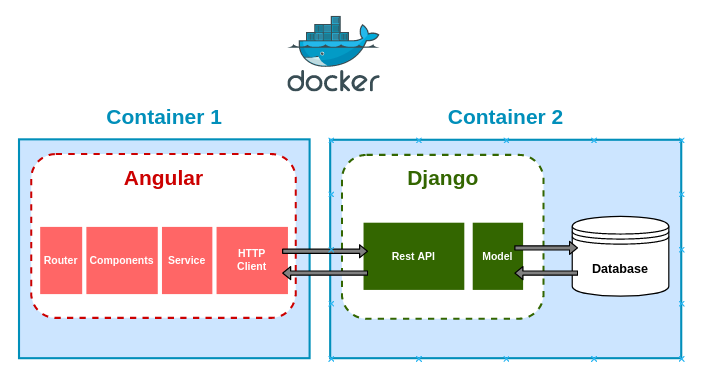
\includegraphics[width=\columnwidth]{./figures/architecture_with_docker}
	\caption{Überblick über die Funktionalität des Technologie-Stacks}
\end{figure}

\newpage
Architekturentscheidungen hier.
Angular als client-side MVC (Architekturprinzip), Architekturstile (micro-service), bestimmtes Vorgehen (user-centered-design)

\section{Fazit und Ausblick}




\begin{thebibliography}{00}
\bibitem{docker} \url{https://www.docker.com/}
\bibitem{angular} \url{https://angular.io/}
\bibitem{django} \url{https://www.django-rest-framework.org/}
\bibitem{mongodb} \url{https://www.mongodb.com/de}
\bibitem{docBox} \url{https://www.doctorbox.de/patienten.jsp}
\bibitem{notion} \url{https://www.notion.so/}
\end{thebibliography}
\end{document}
